\section{Peer-to-Peer-Technologie}
\label{subsec:peer_to_peer_technologie}
% #TODO: Funktion des Kademlia Protokolls nennen und erklären (vielleicht in Grundlagen)
% Im Kademlia-Protokoll sind vier Funktionen definiert, die für die Suche nach
% Knoten und Werten verwendet werden. Diese Funktionen sind \texttt{FIND\_NODE},
% \texttt{FIND\_VALUE}, \texttt{PING} und \texttt{STORE}. Die Funktionen
% \texttt{FIND\_NODE} und \texttt{FIND\_VALUE} werden verwendet, um nach Knoten
% oder Werten zu suchen. Die Funktion \texttt{PING} wird verwendet, um die
% Erreichbarkeit eines Knotens zu überprüfen. Die Funktion \texttt{STORE} wird
% verwendet, um einen Wert in einem Knoten zu speichern.

% Was ist ein Peer-to-Peer-Netzwerk?
% Wie funktioniert es?
% Welche Typen gibt es?
% Welche Vorteile bietet es?
% Welche Nachteile gibt es?
% Welche Anwendungen gibt es?
% Welche Probleme gibt es bei Peer-to-Peer-Netzwerken?
% Welche Lösungen gibt es für diese Probleme?
% Welche Peer-to-Peer-Protokolle gibt es?
% Welche Peer-to-Peer-Protokolle werden in dieser Arbeit verwendet?

Peer-to-Peer-Technologien können in zwei Kategorien unterteilt werden: Peer-to-Peer-Anwendungen und Peer-to-Peer-Infrastrukturen. Die Kategorie der Peer-to-Peer-Anwen-\\dungen umfasst den Dienst der Inhaltsverteilung, bei dem die Teilnehmer Inhalte wie Musik, Videos oder andere Dateien direkt untereinander austauschen \Parencite[730-731]{Khatibi_StructuredUnstructuredP2P}. 

Daher werden viele Peer-to-Peer schnell mit Filesharing in Verbindung bringen, da diese Technologie in der Vergangenheit vor allem dafür genutzt wurde. Das bekannteste Beispiel ist das Filesharing-Netzwerk \textit{Napster}, das 1999 von Shawn \enquote{Napster} Fanning entwickelt wurde. \textit{Napster} war das erste weit verbreitete Filesharing-Netzwerk, das auf Peer-to-Peer-Technologie basierte. Es ermöglichte den Austausch von Musikdateien zwischen den Teilnehmern. Die Musikdateien wurden dabei auf den Computern der Teilnehmer gespeichert und konnten von anderen Teilnehmern heruntergeladen werden. Da diese Art des Datenaustauschs oftmals illegal war, wurde Napster 2001 aufgrund von Urheberrechtsverletzungen abgeschaltet \parencite[S. 4-6]{Mahlmann_P2PNetzwerke}.

Die Peer-to-Peer-Infrastruktur umfasst die Peer-to-Peer-Netzwerke, die für die Kommunikation zwischen den Teilnehmern verwendet werden \parencite[S. 730-731]{Khatibi_StructuredUnstructuredP2P}. Diese Arbeit konzentriert sich auf die Peer-to-Peer-Infrastruktur, die die Kommunikation zwischen den Teilnehmern ermöglichen soll.

Im Instant-Messaging-Bereich repräsentiert das Peer-to-Peer-Modell eine dezentrale Struktur, die dabei hilft, die Kommunikation zwischen den Teilnehmern zu ermöglichen. Im Gegensatz zum Client-Server-Ansatz, bei dem ein zentraler Server die Kommunikation zwischen den Teilnehmern steuert, ermöglicht das Peer-to-Peer-Netzwerk direkte Kommunikation zwischen den Teilnehmern. Beide Modelle bringen Vor- und Nachteile mit sich. Während das Client-Server-Modell eine zentrale Instanz erfordert, um die Kommunikation zu verwalten, ist das Peer-to-Peer-Netzwerk dezentralisiert und benötigt keine solche Instanz. Die Implementierung und Wartung eines Client-Server-Modells gestalten sich einfacher im Vergleich zu einem komplexeren und aufwendigeren Peer-to-Peer-Netzwerk. Das Client-Server-Modell ist weniger flexibel, da es von einer zentralen Instanz abhängt, während das Peer-to-Peer-Netzwerk aufgrund des Fehlens dieser Instanz flexibler ist. Skalierbarkeit ist ebenfalls ein Unterschied: Das Client-Server-Modell ist durch die Kapazität des Servers begrenzt, während das Peer-to-Peer-Netzwerk auf die Kapazität der Teilnehmer zurückgreift, was seine Skalierbarkeit verbessert. In Bezug auf Sicherheit ist das Client-Server-Modell weniger robust, da es auf eine zentrale Instanz angewiesen ist, während das Peer-to-Peer-Netzwerk, das ohne solche Abhängigkeit auskommt, als sicherer gilt \parencite[S. 6-8]{Mahlmann_P2PNetzwerke}.

Nicht jedes Peer-to-Peer-Netzwerk ist gleich. Es gibt verschiedene Typen von Peer-to-Peer-Netzwerken, die sich in ihrer Struktur und Funktionsweise unterscheiden. Abbildung \ref{p2p_typen} zeigt die zwei Haupttypen von Peer-to-Peer-Netzwerken: unstrukturierte und strukturierte Netzwerke \parencite[S. 362-363]{Luntovskyy_ModRechnernetze}.

\begin{center}
    \captionsetup{type=figure}
    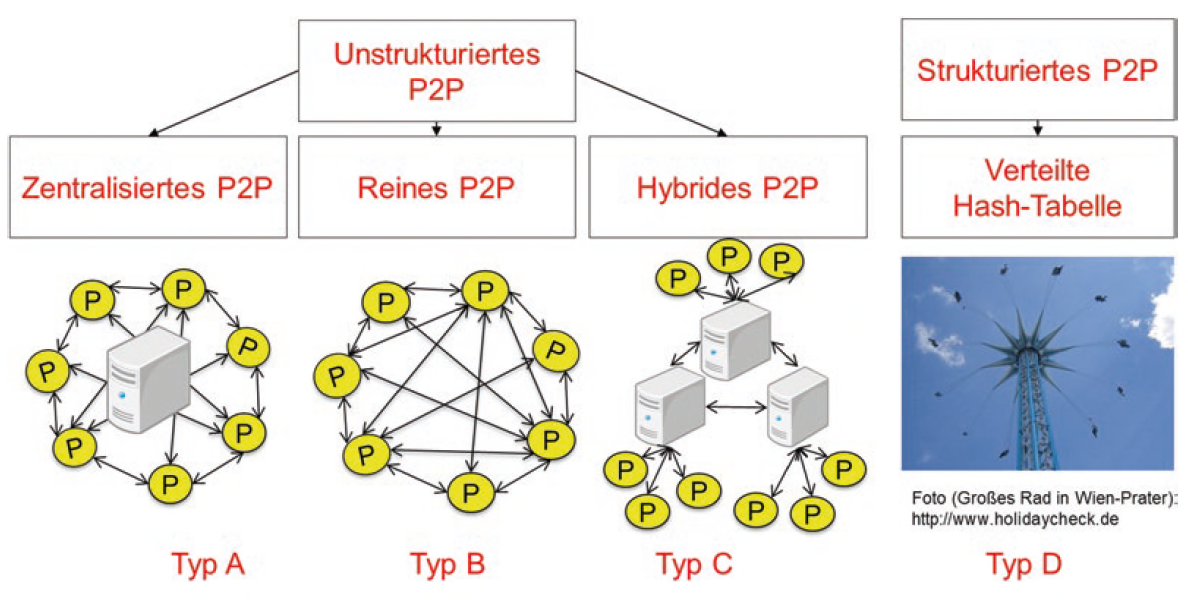
\includegraphics[width=1\linewidth]{images/peer_to_peer_typen.png}
    \captionof{figure}{Typen von Peer-to-Peer-Netzwerken \parencite{Luntovskyy_ModRechnernetze}}
    \label{p2p_typen}
\end{center}

\noindent Unstrukturierte und strukturierte Peer-to-Peer-Netzwerke sind unterschiedliche Ansätze zur Organisation von Knoten und Ressourcen in dezentralen Netzwerken. Unstrukturierte Netzwerke sind charakterisiert durch ihre fehlende explizite Organisationsstruktur, was eine einfache Konnektivität ermöglicht. \textit{Typ A} in Abbildung \ref{p2p_typen} zeigt ein zentralisiertes Netzwerk, was bedeutet, dass alle Teilnehmer mit einem zentralen Server verbunden sind. Als Beispiel für diese Form des Peer-to-Peer dient \textit{Napster}. Bei \textit{Napster} gab es mehrere Server, die die Dateien der Teilnehmer indizierten. Die Teilnehmer konnten Dateien von anderen Teilnehmern herunterladen, indem sie eine Anfrage an einen der Server stellten, der dann die IP-Adresse des Teilnehmers zurückgab, der die Datei zur Verfügung stellte \parencite[S. 170-171]{Saroiu_MeasuringAndAnalyzingNapsterAndGnutellaHosts}. Bei \textit{Typ B} handelt es sich um ein reines Peer-to-Peer-Netzwerk, bei dem die Teilnehmer direkt miteinander verbunden sind. Ein Beispiel für diese Form des Peer-to-Peer ist \textit{Gnutella}. Bei \textit{Gnutella} gab es keine zentrale Instanz, die die Ressourcen der Teilnehmer indizierte. Die Suche nach Ressourcen oder Informationen erfolgt durch Broadcasts oder zufällige Weiterleitungen, was jedoch zu ineffizienten Suchprozessen führen kann, da keine klare Routing-Struktur vorhanden ist \parencite[S. 171]{Saroiu_MeasuringAndAnalyzingNapsterAndGnutellaHosts}. Beim dritten Typ handelt es sich um ein hybrides Peer-to-Peer-Netzwerk, das Elemente aus strukturierten und unstrukturierten Ansätzen kombiniert. Hier agieren einige Teilnehmer als \textit{Super-Nodes}, die die Ressourcen eines Teils aller Teilnehmer indizieren und dadurch als eine Art Server fungieren. Ein Beispiele für diese Form des Peer-to-Peer ist \textit{Gnutella2}\parencite[S. 732]{Khatibi_StructuredUnstructuredP2P}.

Strukturierte Peer-to-Peer-Netzwerke hingegen weisen klare Regeln und Algorithmen zur Organisation der Knoten auf. Diese Netzwerke verfügen über eine explizite Organisationsstruktur, sei es eine Ringstruktur, k-bucket basierte Systeme oder andere, die es ermöglichen, effizientes Routing und eine optimierte Ressourcenverwaltung zu erreichen. Durch diese klar definierte Struktur sind strukturierte Netzwerke oft stabiler und bieten eine effizientere Ressourcenlokalisierung im Vergleich zu ihren unstrukturierten Gegenstücken. Allerdings kann diese Stabilität auf Kosten von Flexibilität und Anpassungsfähigkeit gehen, da Änderungen in der Netzwerktopologie oder hohe Dynamik der Knoten schwerer zu handhaben sind \textcolor{red}{[QUELLE]}.

Hybride Peer-to-Peer-Netzwerke versuchen, das Beste aus beiden Welten zu vereinen, indem sie Elemente aus strukturierten und unstrukturierten Ansätzen kombinieren. Diese Netzwerke integrieren Aspekte einer festen Organisationsstruktur für bestimmte Netzwerkbereiche, während andere Bereiche eher unstrukturiert sind. Als Beispiel hierfür kann Napster genannt werden, das eine oder mehrere Nodes dazu verwendet, um die Inhalte innerhalb des Netzwerks zu indizieren und zu verwalten, während der tatsächliche Download des Inhalts über eine direkte Verbindung zwischen den Teilnehmern erfolgt \parencite{Yang_ComparingHybridP2PSystems}.
Ziel ist es, Flexibilität und Effizienz zu optimieren und gleichzeitig eine gewisse Stabilität zu gewährleisten. Diese hybriden Ansätze streben danach, eine ausgewogene Lösung zu bieten, die sowohl die Anforderungen an eine stabile Struktur als auch an eine dynamische und flexible Umgebung erfüllt, je nach den spezifischen Bedürfnissen und Anwendungsfällen \textcolor{red}{[QUELLE]}.


\begin{itemize}
    \item NAT-Problem erklären (siehe RFC 5128)
    \item Mögliche Lösungen des NAT-Problems (siehe RFC 5128)
    \item Was gibt es so für Protokolle/Algorithmen
    \item (DHTs erklären)
    \item STUN, TURN und ICE erklären (je nach dem, was ich davon verwende)
    \item High Churn
    \item Kademlia vs. Angriffe
\end{itemize}